\section{Introduction}

    \subsection{Cahier des charges}

        \begin{frame}
            \frametitle{Cahier des charges et objectifs}
            \begin{block}{Intitulé du sujet}
                Lecture en clair, grâce à l'utilisation de la réalité augmentée, d'oeuvres réelles préalablement chiffrées et imprimées.
            \end{block}

            \begin{exampleblock}{Conditions}
                \begin{itemize}
                    \item Documentation, définition des niveaux de précision
                    \item Développement itératif
                    \item Comprendre, appliquer nous-même
                \end{itemize}
            \end{exampleblock}
        \end{frame}

    \subsection{Étude bibliographique}

        \begin{frame}
            \frametitle{Méthodes de chiffrement}
            \framesubtitle{Chiffrement symétrique}
            \centering{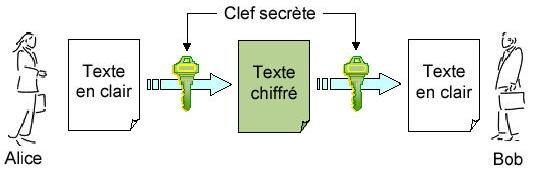
\includegraphics[width=\linewidth]{rsc/symetrique.png}}
            \blfootnote{http://igm.univ-mlv.fr/~dr/XPOSE2007/vma\_PKI/concepts\_de\_base.html}
        \end{frame}

        \begin{frame}
            \frametitle{Méthodes de chiffrement}
            \framesubtitle{Chiffrement asymétrique}
            \begin{columns}
                \begin{column}{.4\linewidth}
                    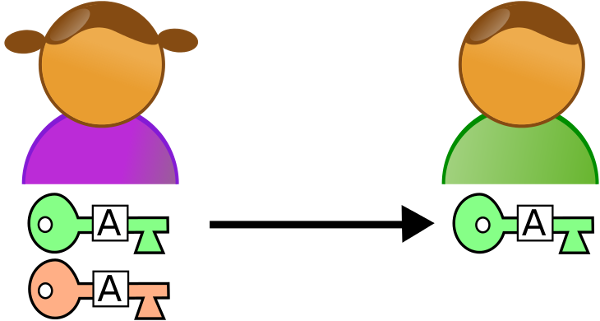
\includegraphics[width=\linewidth]{rsc/asymetrique_1.png}
                \end{column}

                \begin{column}{.4\linewidth}
                    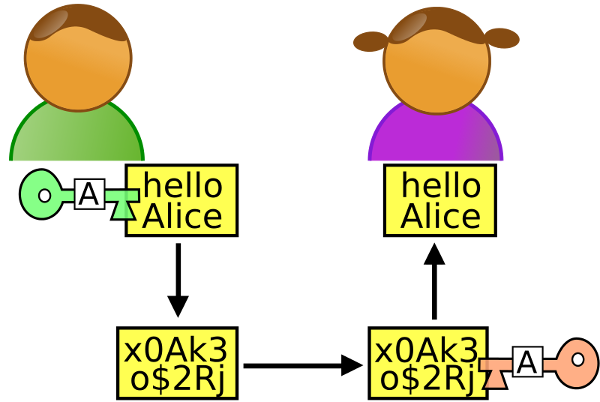
\includegraphics[width=\linewidth]{rsc/asymetrique_2.png}
                \end{column}
            \end{columns}
            \blfootnote{https://fr.wikipedia.org/wiki/Cryptographie\_asymétrique}
        \end{frame}

        \begin{frame}
            \frametitle{Méthodes de chiffrement}
            \framesubtitle{Chiffrement asymétrique avec authentification}
            \centering{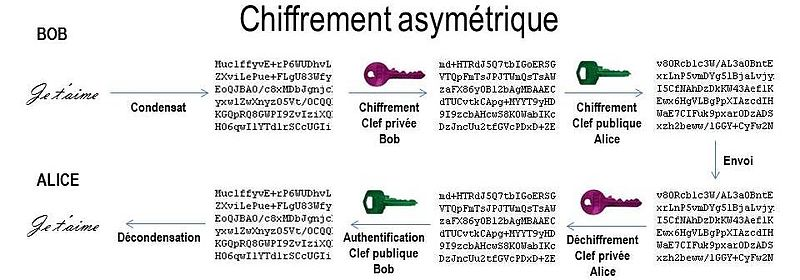
\includegraphics[width=\linewidth]{rsc/authentification.png}}
            \blfootnote{https://fr.wikipedia.org/wiki/Cryptographie\_asymétrique}
        \end{frame}

        \begin{frame}
            \frametitle{Techniques de chiffrement}
            \framesubtitle{Permutation / Substitution}
            \begin{columns}
                \begin{column}{.4\linewidth}
                    \centering{Permutation}
                    \centering{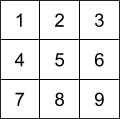
\includegraphics[width=.6\linewidth]{rsc/tab_base.png}}\\
                    \pause
                    \centering{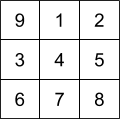
\includegraphics[width=.6\linewidth]{rsc/tab_permutation.png}}
                    \pause
                    \begin{columns}
                        \begin{column}{.5\linewidth}
                            \centering{\textcolor{green}{Rapide}}
                        \end{column}

                        \begin{column}{.5\linewidth}
                            \centering{\textcolor{red}{Moins sécurisée}}
                        \end{column}
                    \end{columns}
                \end{column}

                \begin{column}{.4\linewidth}
                    \centering{Substitution}
                    \pause
                    \centering{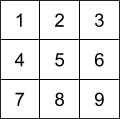
\includegraphics[width=.6\linewidth]{rsc/tab_base.png}}\\
                    \pause
                    \centering{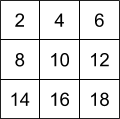
\includegraphics[width=.6\linewidth]{rsc/tab_substitution.png}}
                    \pause
                    \begin{columns}
                        \begin{column}{.5\linewidth}
                            \centering{\textcolor{green}{Robuste}}
                        \end{column}

                        \begin{column}{.5\linewidth}
                            \centering{\textcolor{red}{Sensible au bruit}}
                        \end{column}
                    \end{columns}
                \end{column}
            \end{columns}
        \end{frame}

        \begin{frame}
            \frametitle{Algorithmes de chiffrement}
            \framesubtitle{DES}
            \centering{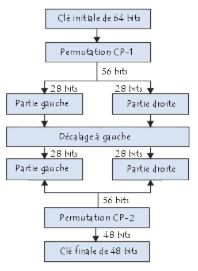
\includegraphics[width=.3\linewidth]{./rsc/des.png}}
            \begin{block}{DES (Data Encryption Standard) - 1977}
                Algorithme de chiffrement symétrique, obsolète.
            \end{block}
            \blfootnote{https://ccm.net/contents/134-introduction-to-encryption-with-des}
        \end{frame}

        \begin{frame}
            \frametitle{Algorithmes de chiffrement}
            \framesubtitle{AES}
            \centering{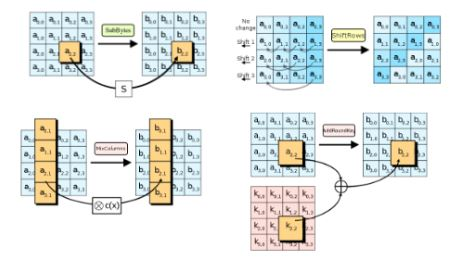
\includegraphics[width=.7\linewidth]{./rsc/aes.png}}
            \begin{block}{AES (Advanced Encryption Standard) - 1997}
                Algorithme de chiffrement symétrique, créé afin de remplacer DES.
            \end{block}
            \blfootnote{http://www.bibmath.net/crypto/index.php?action=affiche\&quoi=moderne/aes}
        \end{frame}

        \begin{frame}
            \frametitle{Algorithmes de chiffrement}
            \framesubtitle{RSA}
            \centering{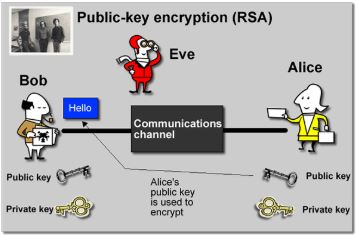
\includegraphics[width=.6\linewidth]{./rsc/rsa.png}}
            \begin{block}{RSA (Rivest Shamir Adleman) - 1983}
                Algorithme de chiffrement asymétrique, clef publique pour chiffrer et clef privée pour déchiffrer.
            \end{block}
            \blfootnote{https://www.boxcryptor.com/fr/encryption/}
        \end{frame}

        \begin{frame}
            \frametitle{Algorithmes de permutation / substitution}
            \framesubtitle{Arnold Transform}
            \centering{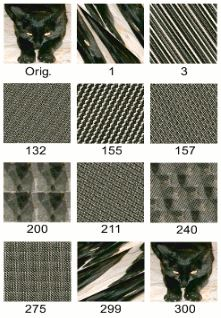
\includegraphics[width=.35\linewidth]{./rsc/arnold.png}}
            \begin{block}{Arnold Transform}
                Algorithme périodique, pas de sécurité. Permutation des pixels :\\
                $P
                \begin{pmatrix}
                    x\\
                    y
                \end{pmatrix}
                =
                \begin{pmatrix}
                    (x + y) mod \mathbb{N}\\
                    (x + 2y) mod \mathbb{N}
                \end{pmatrix}$
            \end{block}
            \blfootnote{https://en.wikipedia.org/wiki/Arnold\%27s\_cat\_map}
        \end{frame}

        \begin{frame}
            \frametitle{Algorithmes de permutation / substitution}
            \framesubtitle{Baker map}
            \centering{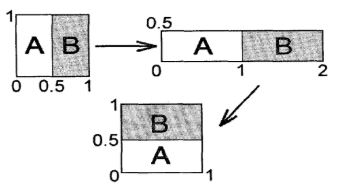
\includegraphics[width=.8\linewidth]{./rsc/baker.png}}
            \begin{block}{Baker map}
                Unit square $\mathbb{I} \times \mathbb{I}$, $\mathbb{I} = \{0, 1\}$\\
                Non périodique.
            \end{block}
            \blfootnote{Image encryption based on chaotic map, Jiri Fridrich, 1997}
        \end{frame}

        \begin{frame}
            \frametitle{(Dé)chiffrement des oeuvres}
            \begin{block}{Méthode choisie}
                \begin{itemize}
                    \item Chiffrement par permutation des positions des pixels (\sout{substitution des valeurs}).
                    \item Générateur chaotique pour définir la nouvelle position des pixels.
                    \item Blocs de pixels (\sout{pixel unique}).
                    \item Blocs moyennés.
                \end{itemize}
            \end{block}
        \end{frame}
